\documentclass{beamer}
%\usetheme{Madrid}
%\usetheme{Boadilla}
%\usetheme{default}
%\usetheme{Warsaw}
%\usetheme{Bergen}
%\usetheme{Frankfurt}
\usetheme{Darmstadt}

%\usecolortheme{seahorse}
%\usecolortheme{beaver}
\usecolortheme[named=orange]{structure}

\setbeamertemplate{footline}[page number]
%\setbeamercovered{transparent}
\setbeamercovered{invisible}
\setbeamertemplate{navigation symbols}{}

\usepackage{multimedia}
\usepackage{graphicx}
\usepackage[utf8]{inputenc}
%\usepackage[T1]{fontenc}
\usepackage[frenchb]{babel} 
\usepackage[all]{xy}
\usepackage{multirow}
\usepackage{lmodern}
\usepackage{subfigure}
\usepackage{ulem}
\usepackage{hyperref}

\usepackage[backend=bibtex]{biblatex}
\addbibresource{papers.bib}

\setbeamertemplate{caption}[numbered] 

%% --------------

\title{Cartographie, localisation et navigation muti-robots utilisant la vision omnidirectionnelle}
\subtitle{Soutenance de Projet de Fin d'\'Etudes}
\author{L\'eo \textsc{Baudouin}\\\emph{leo.baudouin@ifma.fr}}
\institute{
  Institut Pascal (LASMEA)
}
\date{20 septembre 2012}

%% --------------

\begin{document}

\begin{frame}
  \titlepage
  \begin{tabular}{c c c c c}
    \begin{minipage}{0.2\linewidth}
      
\includegraphics[height=10mm]{images/EU.jpg}
    \end{minipage}
    &
    \begin{minipage}{0.2\linewidth}
      
\includegraphics[height=10mm]{images/auvergne.png}
    \end{minipage}
    &
    \begin{minipage}{0.12\linewidth}
      
\includegraphics[height=10mm]{images/logo-IFMA.jpg}
    \end{minipage}
    &
    \begin{minipage}{0.2\linewidth}
      
\includegraphics[height=6mm]{images/logo-LASMEA}
    \end{minipage}
    &
    \begin{minipage}{0.2\linewidth}
      
\includegraphics[height=10mm]{images/logo-IP}
    \end{minipage}
  \end{tabular}
\end{frame}


\begin{frame}{Plan}
  \tableofcontents
\end{frame}

%% --------------

\section{Introduction}
\subsection*{Laboratoire}

\begin{frame}{Institut Pascal}
  \begin{tabular}{l l}
    \begin{minipage}{0.3\linewidth}
      
\includegraphics[width=\linewidth]{images/logo-IP.jpg}
    \end{minipage}
    &
    \begin{minipage}{0.7\linewidth}
      Le laboratoire de l'Institut Pascal est composé de trois équipes regroupant au total une centaine de chercheurs. Le groupe GRAVIR %GRoupe Automatique, VIsion et Robotique
      rassemble trois équipes :
      \begin{itemize}
      \item ComSee %Vision par Ordinateur
      \item Rosace %ROboticS and Autonomous Complex systEms
      \item PerSyst %Systèmes de Perception
      \end{itemize}
    \end{minipage}
  \end{tabular}
\end{frame}


\begin{frame}
  Page 2
\end{frame}

\subsection*{Robotique autonome}

\begin{frame}
  \begin{tabular}{c c}
    \begin{minipage}{0.5\linewidth}
      \begin{figure}
        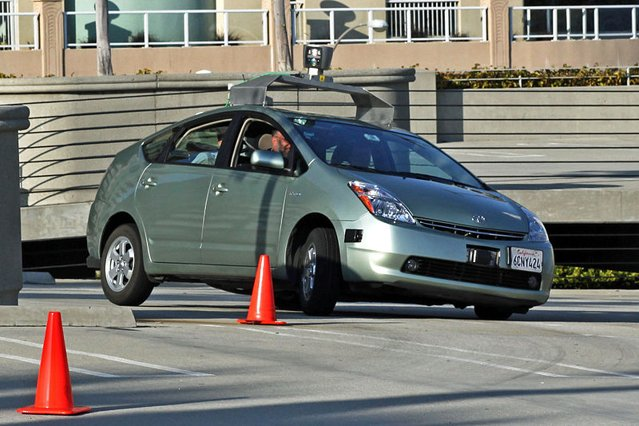
\includegraphics[width=1.0\linewidth]{images/GoogleCar.jpg}
        \caption{Google Car DriverLess}
      \end{figure}
    \end{minipage}
    &
    \begin{minipage}{0.5\linewidth}
      Velodyne LIDAR :
      \begin{itemize}
      \item 64 diodes laser
      \item 1.3 millions de points/secondes
      \item $360$\degre $\times~26.8$\degre
      \item Fragile
      \item 75.000\$
      \end{itemize}
      
      \begin{figure}
      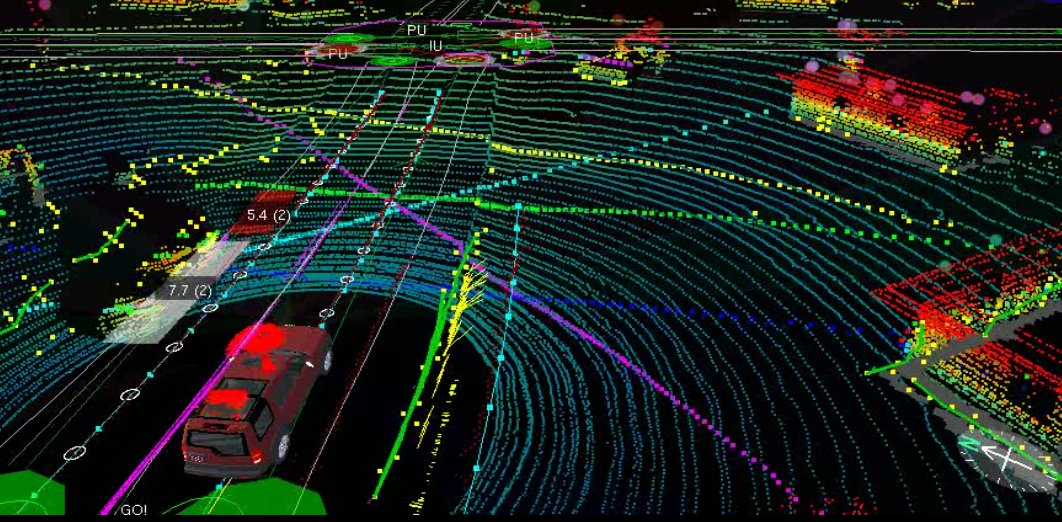
\includegraphics[width=0.8\linewidth]{images/LIDAR.jpg}
      \end{figure}
    \end{minipage}
  \end{tabular}
\end{frame}

\begin{frame}
  \begin{tabular}{c c}
    \begin{minipage}{0.5\linewidth}
      Convoi avec Leader
    \end{minipage}
    &
    \begin{minipage}{0.5\linewidth}
      \begin{figure}
        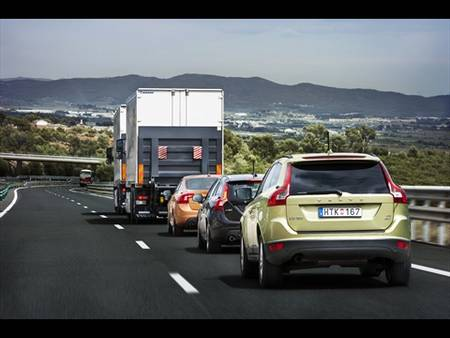
\includegraphics[width=1.0\linewidth]{images/ConvoiVolvo.jpg}
        \caption{Convoi de Volvo autonomes suivant un camion}
      \end{figure}
    \end{minipage}
  \end{tabular}
\end{frame}

\subsection*{Thèse}

\begin{frame}{Projet de thèse}
  \begin{tabular}{c c}
    \begin{minipage}{0.5\linewidth}
      \begin{figure}
        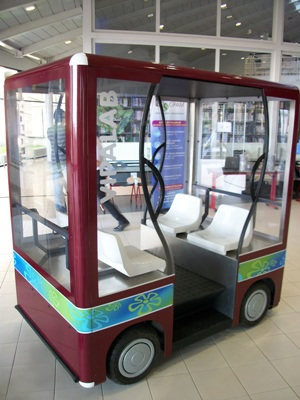
\includegraphics[width=0.8\linewidth]{images/VIPALAB.jpg}
        \caption{Un VipaLab}
      \end{figure}
    \end{minipage}
    &
    \begin{minipage}{0.5\linewidth}
      VipaLab
    \end{minipage}
  \end{tabular}
\end{frame}

\subsection*{Environnement}
\begin{frame}{Tests sur Pavin}

\begin{figure}
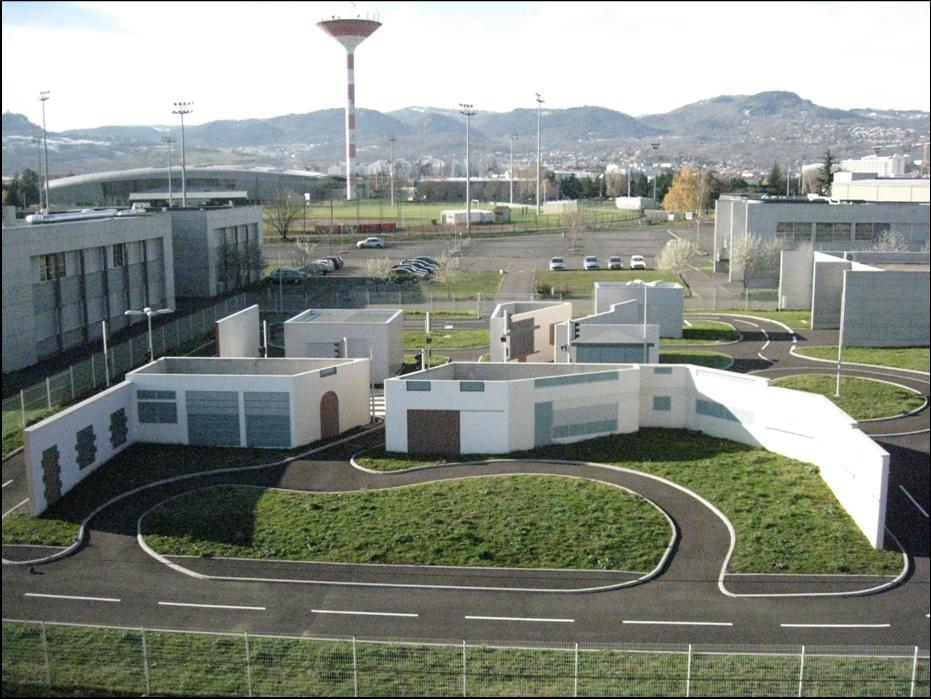
\includegraphics[width=0.7\linewidth]{images/pavin.jpg}
\caption{Espace Pavin pour les simulations grandeur nature}
\end{figure}
% PAVIN is a site dedicated for intelligent urban vehicles. It is composed of 5000m2 space representing typical situation in urban environment: 317m of streets (asphalt) and 264m of open environment (sloppy ground, rough track). 
\end{frame}

\begin{frame}
  Points importants :
  \begin{itemize}
    \begin{small}
    \item Création de carte à partir d'espaces visités par différents robots	
    \item Surveillance d'un environnement dynamique et inconnu	
    \item Lien entre la vision omnidirectionelle et le controle stratégique coopératif	
    \item Utilisation d'informations visuelles comme les informations mutuelles	
    \item Utilisation de cartes topologiques à l'aide de capteurs externes	
    \item Localisation par l'apparence et/ou par la 3D	
    \item Localisation inter-robot, entre-aide	
    \item Formation avec ou sans leader	
    \item Suivi d'une cible à l'aide de plusieurs robots
    \end{small}
  \end{itemize}
\end{frame}

%% --------------

\section{Recherche}
\subsection*{Méthodes}

\begin{frame}{Recherche bibliographique}
  \begin{itemize}
  \item Comment chercher ?
  \item Comment trouver ?
  \item Disponibilité ?
  \item Achats ?
  \item Aller de publi en publi...
  \item Trouver des vidéos sur le net ...
  \item Site web ...
  \item Notions de maths dans les thèses
  \end{itemize}
\end{frame}


\subsection*{Gestion Bibliographique}

\begin{frame}{Bibliographie}

  \begin{itemize}
  \item Buts et objectifs
  \item Intérêts %Reconnaissance
    %\item Reconnaissance
  \item Inconvénients
    \vspace{5mm}
  \item Contenu : %(121 ouvrages) :
    \begin{itemize}
    \item 3 livres
    \item 11 thèses
    \item 30 articles de journaux
    \item 74 conférences
    \item 3 autres
    \end{itemize}
  \end{itemize}
\end{frame}

\begin{frame}
  \begin{figure}
    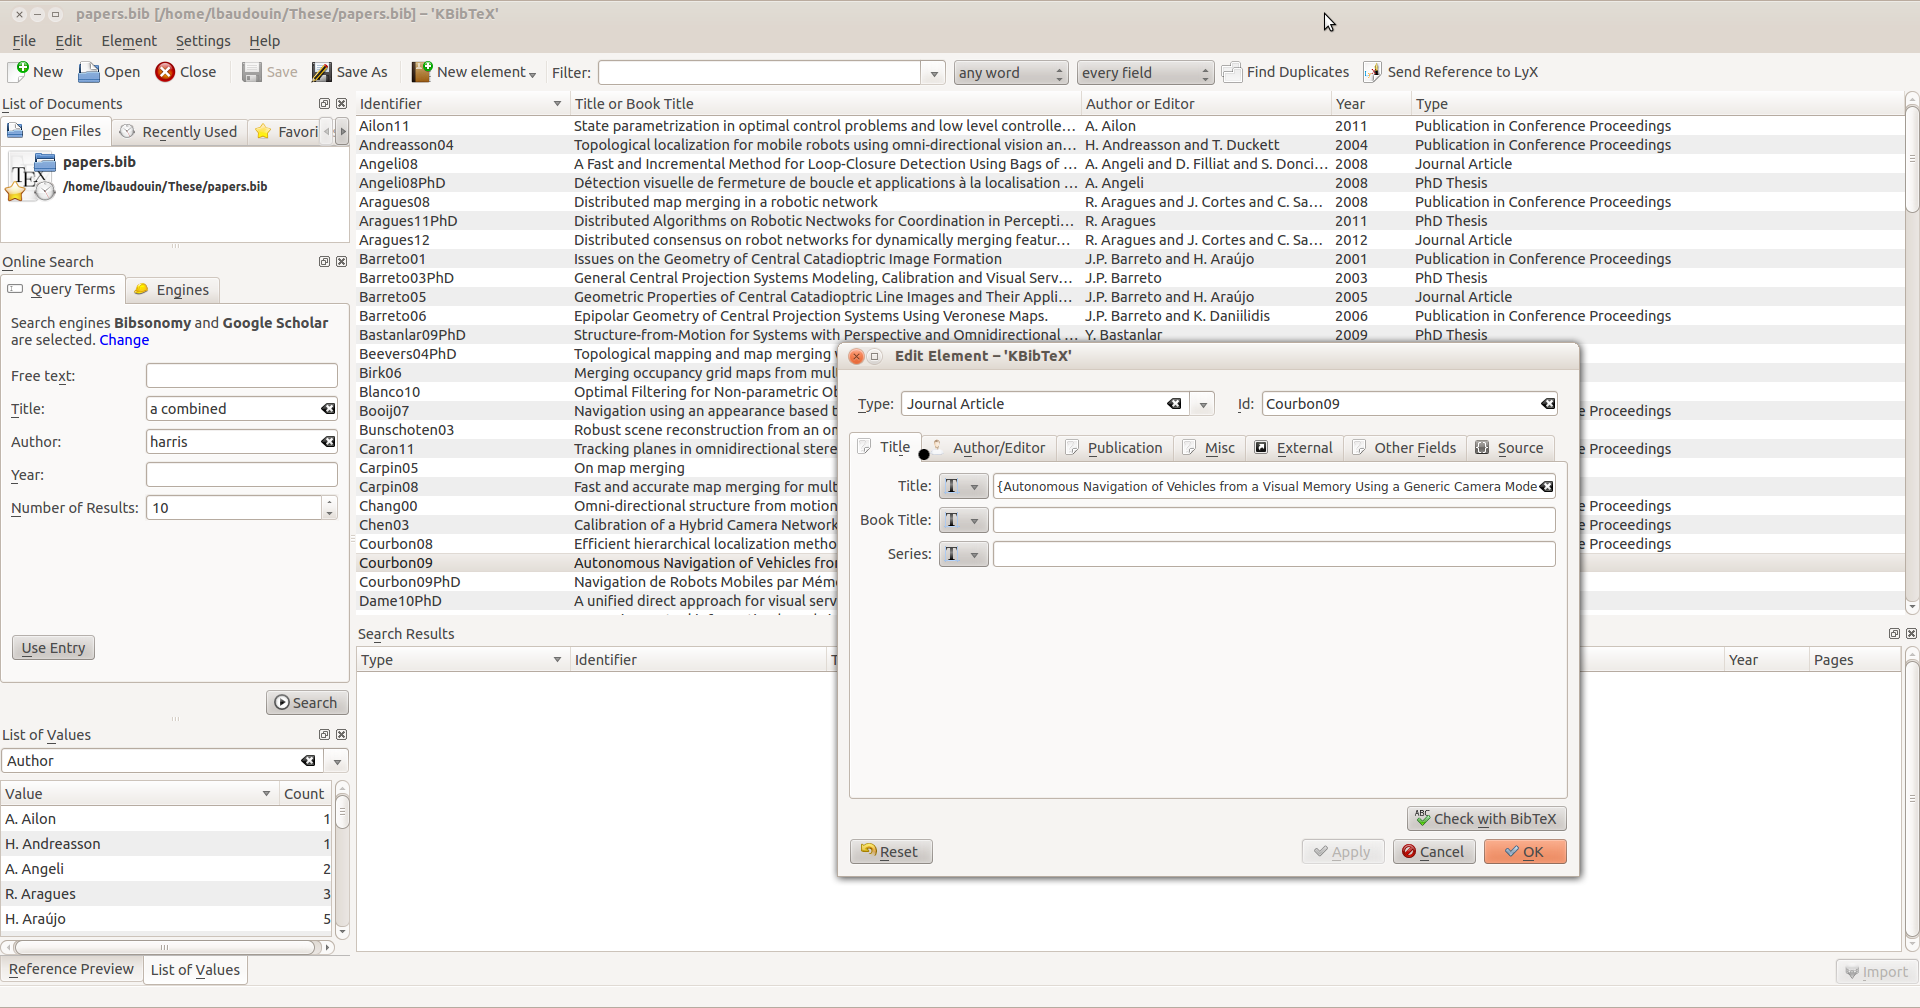
\includegraphics[width=1.0\linewidth]{images/KBibTex.png}
    \caption{Capture d'écran de KBibTex, ligiciel libre de gestion de bibliographie}
  \end{figure}
\end{frame}

\subsection*{Articles}

\begin{frame}{Exemple}
  %Auteurs, écriture, publication (tro, iros, \dots)

  Exemple :\\
  \vspace{2mm}
  %\begin{tiny}
  \begin{scriptsize}
    @inproceedings$\lbrace$ baudouin:humanoids:11,\\
    \hspace{5mm} author = "L. Baudouin and N. Perrin and T. Moulard and F. Lamiraux and O. Stasse and E. Yoshida",\\
    \hspace{5mm} booktitle = "\{IEEE/RAS International Conference on Humanoid Robotics (Humanoids'11)\}",\\
    \hspace{5mm} title = "\{Real-time Replanning Using 3D Environment for Humanoid Robot\}",\\
    \hspace{5mm} url = "http://ubuntuone.com/6zyz487WVECpyW88tEfQz5",\\
    \hspace{5mm} year = "2011"\\
    \vspace{-2mm}
    $\rbrace$
  \end{scriptsize}
  %\end{tiny}
  \vspace{5mm}

  Article :\\
  \begin{scriptsize}
    \mbox{
      \citeauthor{baudouin:humanoids:11}
      \citetitle{baudouin:humanoids:11}
      \cite{baudouin:humanoids:11}
    }
  \end{scriptsize}
  %\vspace{5mm}

  Thèse :\\
  \begin{scriptsize}
    \mbox{
      \citeauthor{Courbon09PhD}
      \citetitle{Courbon09PhD}
      \cite{Courbon09PhD}}
  \end{scriptsize}
  \vspace{5mm}

\end{frame}

\begin{frame}{Bibliographie}
  %\begin{minipage}{0.5\linewidth}
  \printbibliography[heading=none]
  %\end{minipage}
\end{frame}

%% --------------

\section{Avancement}

\subsection*{Vision}
\begin{frame}{Reconstruction 3D}
  \begin{tabular}{c c}
    \begin{minipage}{0.5\linewidth}
      \begin{figure}
        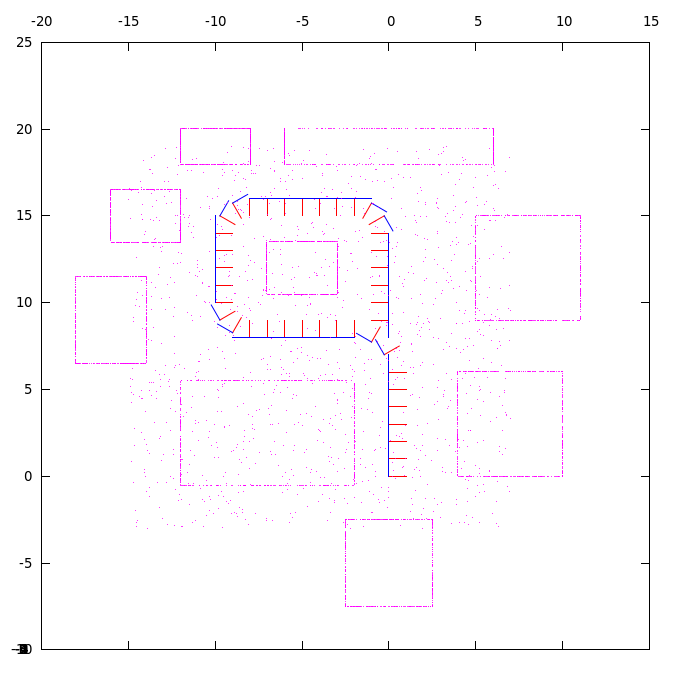
\includegraphics[width=0.9\linewidth]{images/createimages.png}
        \caption{Simulation d'un environnement}
      \end{figure}
    \end{minipage}
    &
    \begin{minipage}{0.5\linewidth}
      \begin{figure}
        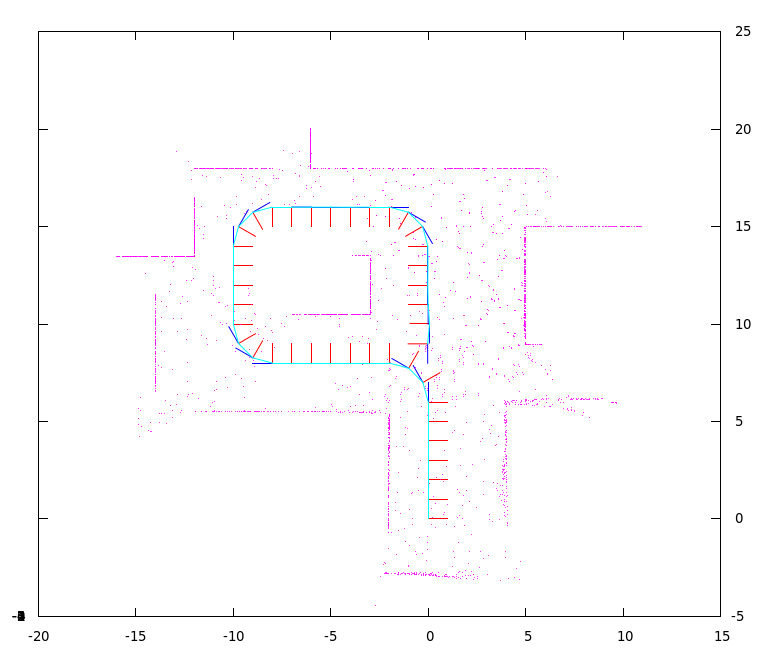
\includegraphics[width=1.0\linewidth]{images/buildfromvideo.png}
        \caption{Reconstruction à partir des points 2D}
      \end{figure}
    \end{minipage}
  \end{tabular}
\end{frame}

\subsection*{Création de cartes}
\begin{frame}{Développement}
Programmes ou librairies testés :
\begin{itemize}
  \item Sovin
  \item loop\_closure
  \item SSBA (Simple Sparse Bundle Adjustment)
  \item RobotVision
  \item ScaViSLAM
  \item MRPT
\end{itemize}
\end{frame}

\subsection*{Navigation}
\begin{frame}

\end{frame}

\subsection*{Situation actuelle}
\begin{frame}{Problèmes rencontrés}
  Retard
\end{frame}

%% --------------

\section{Conclusion}
\subsection*{Objectifs}
\begin{frame}{Suite des travaux}
  \begin{tabular}{c c}
    \begin{minipage}{0.5\linewidth}
      A mettre en place en deux ans :
      \begin{enumerate}
      \item Navigation Classique
      \item Navigation Topologique %Graphe : Noeuds + distance (arc)
      \item Mise en Formation
      \item Déplacements en Formation
      \item Survaillance \& Suivi de Cible
      \end{enumerate}
    \end{minipage}
    &
    \begin{minipage}{0.5\linewidth}
      \begin{figure}
        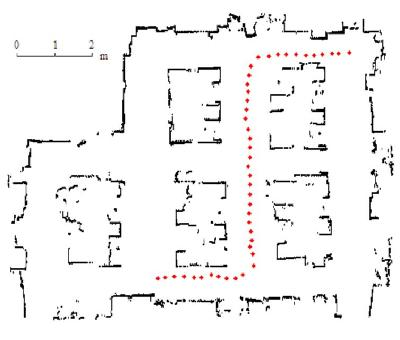
\includegraphics[width=0.8\linewidth]{images/navigation.jpg}\\
        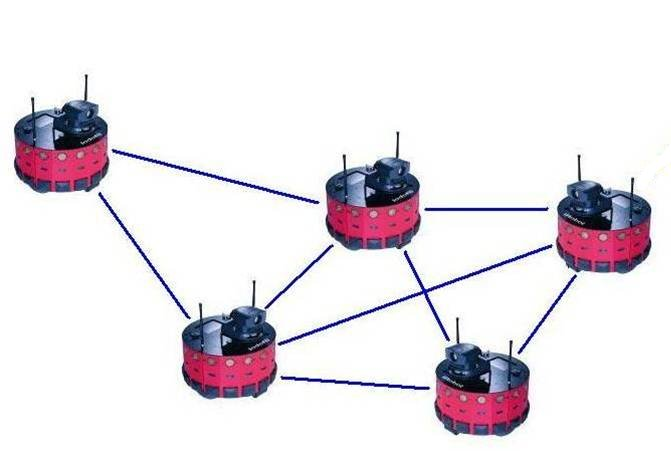
\includegraphics[width=0.8\linewidth]{images/formation.jpg}
      \end{figure}
    \end{minipage}
  \end{tabular}

\end{frame}

\subsection*{Six mois de Stage}
\begin{frame}{Conclusion}
  \begin{figure}
    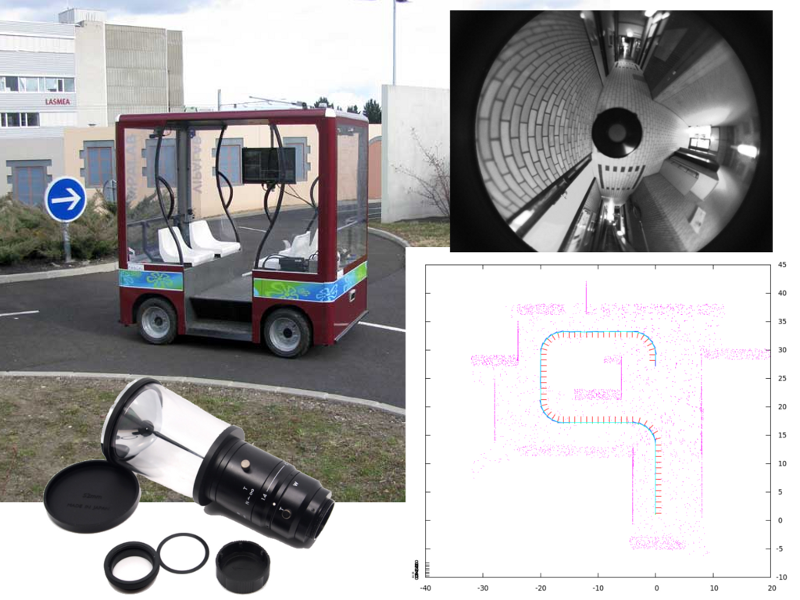
\includegraphics[width=0.7\linewidth]{images/conclusion.png}
  \end{figure}
\end{frame}


\end{document}  
